\documentclass[12pt]{article}
\usepackage{tabularx}
\usepackage{amsmath} 
\usepackage{graphicx}
\usepackage[margin=1in]{geometry}
\usepackage{cite}
\usepackage[final]{hyperref}
\hypersetup{
	colorlinks=true,      
	linkcolor=blue,       
	citecolor=blue,       
	filecolor=magenta,    
	urlcolor=blue         
}
\usepackage{blindtext}
\usepackage{amssymb}
\usepackage{esint}
\usepackage{tikz}
\usepackage{pgfplots}
\usepackage{gensymb}
\usetikzlibrary{datavisualization}
\usetikzlibrary{datavisualization.formats.functions}
\newcommand{\Prho}{.8}%
\newcommand{\Ptheta}{55}%
\newcommand{\Pphi}{60}%
\usepackage{tikz-3dplot}
\newcommand{\uvec}[1]{\boldsymbol{\hat{\textbf{#1}}}}
%++++++++++++++++++++++++++++++++++++++++
\usepackage{empheq}

\newcommand*\widefbox[1]{\fbox{\hspace{2em}#1\hspace{2em}}}

\begin{document}

\usetikzlibrary{scopes}
\def\iangle{35} % Angle of the inclined plane

\def\down{-90}
\def\arcr{0.5cm} % Radius of the arc used to indicate angles

\title{ECE 3030 - HW 10}
\author{Joshua Tensuan - jvt24}
\date{December 6, 2022}
\maketitle

One slip day used.

\begin{enumerate}
	\item [10.1]
	\begin{enumerate}
		\item [(a)]
		The current density phasors of each dipole are given by,
		\[\vec J_1(\vec r)=\hat z Id\delta^3\left(\vec r-\hat z \frac{h}{2}\right)\]
		\[\vec J_2(\vec r)=-\hat z Id\delta^3\left(\vec r +\hat z\frac{h}{2}\right)\]
		The radiated waves from dipole 2 travel $h\cos(\theta)$ more than the radiated waves from dipole 1.
		Thus, the waves from dipole 2 accumulates $kh\cos(\theta)$ more phase.
		We also know that since $\alpha=-\pi$, that the waves from dipole 2 lag behind by a phase of $\pi$.
		Thus, the total phase difference of the radiated waves, $\Delta \phi$, is given by,
		\[\Delta\phi = kh\cos(\theta)-\pi\]
		If we want to find the maxima, we want constructive interference where, $\Delta\phi = kh\cos(\theta)-\pi = n2\pi$ where $n\in\mathbb{Z}$.
		Substituting in $k=2\pi/\lambda$ and $h=\lambda/2$,
		\[\frac{2\pi}{\lambda}\frac{\lambda}{2}\cos(\theta)-\pi =n 2\pi\]
		\[\to \cos(\theta)-1=2n\to \cos(\theta)=2n+1\]
		Since the range of $\cos(\theta)=[-1,1]$, we know that we will only have solutions for $n=-1,0$.
		Then, the angular locations of the maxima, $\theta_{\mathrm{max}}$ are given by,
		\[\cos(\theta_{\mathrm{max}})=\{-1,1\}\]
		\[\theta_{\mathrm{max}} = -\pi, 0\]
		Similarly, if we want to find the nulls, we want total destructive interference where, $\Delta\phi = kh\cos(\theta)-\pi = (2m+1)\pi$ where $m\in\mathbb{Z}$.
		Substituting in $k=2\pi/\lambda$ and $h=\lambda/2$,
		\[\frac{2\pi}{\lambda}\frac{\lambda}{2}\cos(\theta)-\pi=(2m+1)\pi\]
		\[\to \cos(\theta)-1 = 2m+1\to \cos(\theta)=2m+2\]
		Since the range of $\cos(\theta)=[-1,1]$, we know that we will only have solutions for $m=-1$.
		Then, the angular locations of the minima, $\theta_{\mathrm{min}}$ are given by,
		\[\cos(\theta_{\mathrm{min}})=\{0\}\]
		\[\theta_{\mathrm{min}} = \pi/2\]
		\[\boxed{\begin{cases}
			\theta_{\mathrm{max}} = -\pi, 0 \\ 
			\theta_{\mathrm{min}} = \pi/2	
		\end{cases}}\]

		\item [(b)]
		Using the principle of superposition, we can find the far-field of the electric field to be,
		\[\vec E_{\mathrm{ff}}(\vec r)=\hat \theta\frac{j\eta_0kId}{4\pi r}\sin(\theta)e^{-jkr}\left[e^{jk\frac{h}{2}\cos(\theta)}-e^{-jk\frac{h}{2}\cos(\theta)}\right]\]
		\[\vec E_{\mathrm{ff}}(\vec r)=\hat \theta\frac{j\eta_0kId}{4\pi r}\sin(\theta)e^{-jkr}\left[e^{jk\frac{h}{2}\cos(\theta)}-e^{-jk\frac{h}{2}\cos(\theta)}\right]\]
		and the far-field of the magnetic field to be,
		\[\vec H_{\mathrm{ff}}(\vec r)=\hat \phi\frac{jkId}{4\pi r}\sin(\theta)e^{-jkr}\left[e^{jk\frac{h}{2}\cos(\theta)}-e^{-jk\frac{h}{2}\cos(\theta)}\right]\]
		Then, the time-averaged Poynting vector is given by,
		\[\left\langle \vec S(\vec r, t)\right\rangle=\frac{1}{2}\mathrm{Re}\left[\vec E_{\mathrm{ff}}(\vec r)\times \vec H_{\mathrm{ff}}^*(\vec r)\right]\]
		\[\vec E_{\mathrm{ff}}(\vec r)\times \vec H^*_{\mathrm{ff}}(\vec r)=\begin{vmatrix}
			\hat r & \hat \theta & \hat \phi \\ 
			0 & E_{\mathrm{ff}}(\vec r) & 0 \\ 
			0 & 0 & -H_{\mathrm{ff}}(\vec r)

		\small

		\end{vmatrix}=\hat r\eta_0\left(\frac{kId}{4\pi r}\right)^2\sin^2(\theta)\left(e^{jk\frac{l}{2}\cos(\theta)}-e^{-jk\frac{l}{2}\cos(\theta)}\right)^2\]

		\normalsize

		Then,
		\[\left \langle \vec S(\vec r, t)\right \rangle \cdot \hat r  =\frac{1}{2}\eta_0\left(\frac{kId}{4\pi r}\right)^2\sin^2(\theta)\cdot \mathrm{Re}\left[\left(e^{jk\frac{l}{2}\cos(\theta)}-e^{-jk\frac{l}{2}\cos(\theta)}\right)^2\right]\]
		\[P_{\mathrm{rad}}=\iint \left \langle \vec S(\vec r ,t)\right \rangle \cdot d\vec A\]
		Through Mathematica, we find that the gain is given by,
		\[G(\theta,\varphi)\propto\sin^2(\theta)\left(\frac{2+2\cos\left[\pi\cos(\theta)+\pi\right]}{4}\right)\]
		Then, the radiation pattern is given by,
		\[p(\theta,\varphi)=\left(\frac{1+\cos\left[\pi\cos(\theta)+\pi\right]}{2}\right)\]
		Plotting this in Python yields,

		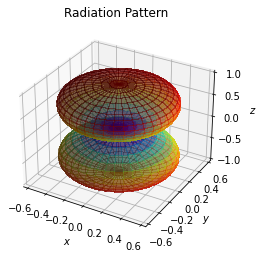
\includegraphics[width = 5in]{images/q1-1.png}

		This plot verifies my answers in part a because the maxima are obtained on the $z$-axis ($\theta_{\mathrm{max}}=-\pi,0$) and the minima are obtained on the $xy$-plane ($\theta_{\mathrm{min}}=\pi/2$).

		
	\end{enumerate}

	\item [10.2]
	\begin{enumerate}
		\item [(a)]
		% Suppose the left-most Hertzian dipole element corresponds to the $n=0$-th element and the right-most Hertzian dipole element corresponds to the $n=N-1$-th element.
		% We know that the waves radiated from the $n$-th dipole element travel a distance $d\sin(\theta)\cos(\phi)$ less than the $n-1$-th dipole element.
		% Thus, between each dipole, a phase of $kd\sin(\theta)\cos(\phi)$ is picked up.
		% Additionally, each dipole has a phase difference of $\alpha$.
		% Thus, the total phase difference of the radiated waves of the array, $\Delta \phi$, is given by,
		% \[\Delta \phi = \sum_{m=0}^{N-1}m(kd\sin(\theta)\cos(\phi)+\alpha)\]
		% Using the formula for arithmetic sums,
		% \[\Delta \phi =\frac{N}{2}[(N-1)(kd\sin(\theta)\cos(\phi)+\alpha)]\]
		% To find the maxima, we set the phase difference to an integer multiple of $2\pi$.
		% \[\Delta \phi =\frac{N}{2}[(N-1)(kd\sin(\theta)\cos(\phi)+\alpha)]=2m\pi, \; m \in \mathbb{Z}\]

		Suppose the left-most Hertzian dipole element corresponds to the $n=0$-th element and the right-most Hertzian dipole element corresponds to the $n=N-1$-th element.
		We know that the waves radiated from the $n$-th dipole element travel a distance $d\sin(\theta)\cos(\phi)$ less than the $n-1$-th dipole element.
		Thus, between each dipole, a phase of $kd\sin(\theta)\cos(\phi)$ is picked up.
		Additionally, each dipole has a phase difference of $\alpha$.
		Thereby, the total phase difference of the radiated waves, $\Delta \phi$, is given by,
		\[\Delta \phi = ka\sin(\theta)\cos(\phi)+\alpha\]
		If we want complete constructive interference (a maximum), we want $\Delta\phi = 2m\pi$ where $m$ is any arbitrary integer.
		Thus, the equation becomes,
		\[ka\sin(\theta)\cos(\phi)+\alpha = 2m\pi\]
		If we want to have a single lobe around $\phi = 0$, we want it so that the above equation is only satisfied when $\sin(\theta)\cos(\phi)$ are at their maximum values.
		Additionally, we would want to find solutions for $m=0$.
		This ensures that there can be no "aliasing" where different values for $\theta$ and $\phi$ could yield similar complete constructive interference solutions.
		Thus, we end up with,
		\[ka=-\alpha\]
		Substituting in relevant terms,
		\[\boxed{\frac{2\pi}{\lambda}d=-\alpha}\]

		\item [(b)]
		Finding $\alpha$ using our conclusion from part a,
		\[\alpha = -\frac{2\pi}{\lambda}d=-\frac{2\pi}{\lambda}\frac{\lambda}{4}=-\frac{\pi}{2}\]
		We know that in general, the total far-field electric field is a superposition of the electric field of the individual dipole elements.
		Thus,
		\[\vec E_{\mathrm{ff}}(\vec r)=\vec E(r,\theta,\phi)\sum_{m=0}^{N-1}e^{jm\alpha}e^{jk\hat r \cdot \vec h_m}=\vec E(r,\theta,\phi)F(\theta,\phi)\]
		The array factor, $F(\theta,\phi)$ is given by,
		\[F(\theta,\phi)=e^{jk\hat r \cdot \vec h_0}\sum_{m=0}^{N-1}e^{j\alpha m}e^{jka\sin(\theta)\cos(\phi)m}\]
		Using the formula of a geometric series, we find that,
		\[|F(\theta,\varphi)|^2=\frac{\sin^2\left[\frac{N}{2}(\alpha + ka\sin(\theta)\cos(\phi))\right]}{\sin^2\left[\frac{1}{2}(\alpha+ka\sin(\theta)\cos(\phi))\right]}\]
		Substituting in $\alpha = -\pi/2$, $ka=-\alpha$, and $N=20$,
		\[|F(\theta,\phi)|^2 = \frac{\sin^2\left[10\left(-\frac{\pi}{2}+\frac{\pi}{2}\sin(\theta)\cos(\phi)\right)\right]}{\sin^2\left[\frac{1}{2}\left(-\frac{\pi}{2}+\frac{\pi}{2}\sin(\theta)\cos(\phi)\right)\right]}=\frac{\sin^2\left[-5\pi+5\pi\sin(\theta)\cos(\phi)\right]}{\sin^2\left[-\frac{\pi}{4}+\frac{\pi}{4}\sin(\theta)\cos(\phi)\right]}\]
		Then, from lecture, we derived that the resulting radiation pattern is,
		\[p(\theta,\phi)=\frac{1}{N^2}\sin^2(\theta)|F(\theta,\phi)|^2\]
		Plotting this in Python yields,

		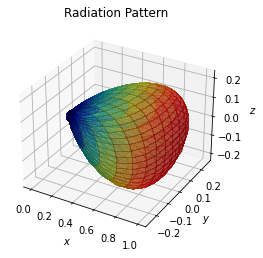
\includegraphics[width = 5in]{images/q2-1.png}

		\item [(c)]
		Finding $\alpha$,
		\[\alpha=-\left(kd+\frac{\pi}{N}\right)=-\left(\frac{2\pi}{\lambda}\frac{\lambda}{4}+\frac{\pi}{20}\right)=-\frac{11\pi}{20}\]
		Substituting this into $|F(\theta,\phi)|^2$,
		\[|F(\theta,\phi)|^2=\frac{\sin^2\left[10\left(-\frac{11\pi}{20}+\frac{\pi}{2}\sin(\theta)\cos(\phi)\right)\right]}{\sin^2\left[\frac{1}{2}\left(-\frac{11\pi}{20}+\frac{\pi}{2}\sin(\theta)\cos(\phi)\right)\right]}\]
		The radiation pattern is then given as,
		\[p(\theta,\phi)=\frac{1}{N}\sin^2(\theta)|F(\theta,\phi)|^2\cdot \frac{1}{N^{-1}\cdot |F(\theta,\phi)|^2_{\mathrm{max}}}\]
		\[p(\theta,\phi)=\sin^2(\theta)\frac{|F(\theta,\phi)|^2}{|F(\theta,\phi)|^2_{\mathrm{max}}}\]
		Plotting this in Python yields,

		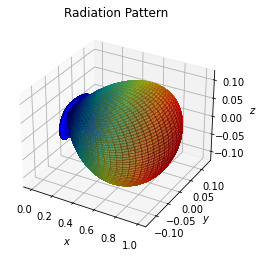
\includegraphics[width = 5in]{images/q2-2.png}

		\item [(d)]
		The antenna with the Hansen-Woodyard condition (antenna from part c) is more directive.
		This is evidenced by the fact that the main lobe in part c is more narrow than in part d.
		For instance, the main lobe in part c only ranges from $z:[-0.05,0.05]$ while the main lobe in part d ranges from $z:[-0.1,0.1]$.
		However, this comes at the cost of the lobe in part c having more of its power in its side lobes.

		Plotting the radiation pattern on the $xy$-plane to find the angular width of the main lobe,

		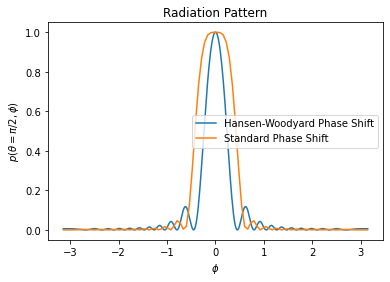
\includegraphics[width=5in]{images/q2-3.png}

		We find that roughly (via the graph), with the standard phase shift, the radiation pattern has its first nulls on $\phi=\pm 0.73$ and that with the Hansen-Woodyard phase shift, the radiation pattern has its first nulls on $\phi=\pm 0.45$.

		We can further narrow the lobe without introducing additional lobes by adding more Hertzian dipoles in the array.
		Additionally, we could also narrow the lobe by decreasing the wavelength of the radiated emission (while still maintaining the same conditions on the phase shifts between each Hertzian dipole in the array).

		\item [(e)]
		Finding the $\alpha$ for the standard phase shift when we double the antenna separation from $d=\lambda/4 \to \lambda/2$,
		\[\alpha = -\frac{2\pi}{\lambda}d = -\frac{2\pi}{\lambda}\frac{\lambda}{2}=-\pi\]
		Substituting in $\alpha = -\pi$, $ka=-\alpha$, and $N=20$ to our previous formulas for the array factor and radiation pattern,
		\[|F(\theta,\phi)|^2 = \frac{\sin^2\left[10\left(-\pi+\pi\sin(\theta)\cos(\phi)\right)\right]}{\sin^2\left[\frac{1}{2}\left(-\pi+\pi\sin(\theta)\cos(\phi)\right)\right]}\]
		\[p(\theta,\phi)=\frac{1}{N^2}\sin^2(\theta)|F(\theta,\phi)|^2\]
		Plotting this in Python yields,

		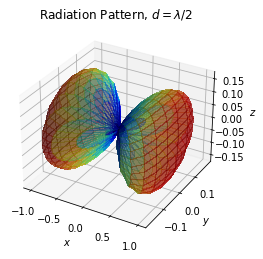
\includegraphics[width = 5in]{images/q2-4.png}

		Finding $\alpha$ for the Hansen-Woodyard phase shift,
		\[\alpha=-\left(kd+\frac{\pi}{N}\right)=-\left(\frac{2\pi}{\lambda}\frac{\lambda}{2}+\frac{\pi}{20}\right)=-\frac{21\pi}{20}\]
		Substituting this into $|F(\theta,\phi)|^2$,
		\[|F(\theta,\phi)|^2=\frac{\sin^2\left[10\left(-\frac{21\pi}{20}+\pi\sin(\theta)\cos(\phi)\right)\right]}{\sin^2\left[\frac{1}{2}\left(-\frac{21\pi}{20}+\pi\sin(\theta)\cos(\phi)\right)\right]}\]
		Then, the radiation pattern is given as,
		\[p(\theta,\phi)=\sin^2(\theta)\frac{|F(\theta,\phi)|^2}{|F(\theta,\phi)|^2_{\mathrm{max}}}\]

		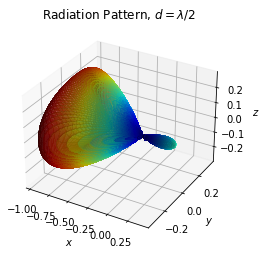
\includegraphics[width=5in]{images/q2-5.png}

		This change is not beneficial for point-to-point communications between two antennas because the power radiated is more "spread out".
		For instance, with the standard phase shift, two main lobes are created with this change, which results in power being more "spread out" as it radiates away from the antenna.
		Further, with the Hansen-Woodyard condition, we notice that the main lobe has actually increased in size, ranging from $z:(-0.2,0.2)$.

	\end{enumerate}

	\item [10.3]
	\begin{enumerate}
		\item [(a)]
		The Friis transmission equation tells us that for a matched transmitter and receiver antenna system,
		\[\frac{P_{\mathrm{out}}}{P}=\eta_pG_1(\theta_1,\phi_1)G_2(\theta_2,\phi_2)\left(\frac{\lambda}{4\pi L}\right)^2\]
		Assuming no polarization mismatch, $\eta_p=1$.
		Then, finding $G_2$,
		\[\frac{P_{\mathrm{out}}}{P}\cdot \frac{1}{G_1(\theta_1,\phi_1)}\cdot \left(\frac{4\pi L}{\lambda}\right)^2=G_2(\theta,\phi_2)\]
		Substituting in numbers, we find that, (use $L\approx 14.8\cdot 10^9\:\mathrm{mi}=2.39\cdot 10^{13}\:\mathrm{m}$ and $\lambda =c/f = 0.0357\:\mathrm{m}$)
		\[G_2(\theta,\phi_2)=\frac{1\cdot 10^{-3}\cdot 10^{-145/10}}{20}\cdot \frac{1}{10^{4.8}}\cdot\left(\frac{4\pi \cdot (2.39\cdot 10^{13})}{0.0357}\right)^2\]
		\[G_2(\theta,\phi_2)=1.77\cdot 10^8\]
		Converting this to decibels,
		\[G_2(\theta,\phi_2)=10\cdot \log_{10}\left(1.77\cdot 10^8\right)=82.5 \: \mathrm{dB}\]
		\[\boxed{G_2(\theta,\phi)=82.5\:\mathrm{dB}}\]

		\item [(b)]
		To find how long the probe travels before the receiver drops below $-200\:\mathrm{dBm}$, we can just back-solve the Friis transmission equation for $L$.
		\[\frac{P_{\mathrm{out}}}{P}=G_1(\theta_1,\phi_1)G_2(\theta_2,\phi_2)\left(\frac{\lambda}{4\pi L}\right)^2\]
		Substituting in variables,
		\[\frac{1\cdot 10^{-3}\cdot 10^{-200/10}}{20}=10^{4.8}\cdot 10^{8.25}\cdot \left(\frac{0.0357}{4\pi \cdot L}\right)^2\]
		Through trivial algebra, we find that,
		\[L=1.344 \cdot 10^{16}\:\mathrm{m}\]
		Thus, the probe could travel $1.341\cdot 10^{16}\:\mathrm{m}$ more until it reaches its destination.
		\[\boxed{L=1.344 \cdot 10^{16}\:\mathrm{m}, \; \Delta 1.341\cdot 10^{16}\:\mathrm{m}}\]
		This would be easily within the reach of the Oort cloud which is $L=3\cdot 10^{11}\:\mathrm{km}=3\cdot 10^{14}\:\mathrm{m}$ away from the Earth.


	\end{enumerate}

	\item [10.4]
	\begin{enumerate}
		\item [(a)]
		In lecture, we determined that if the dipole is very thin, the reactance goes to $0$ at $d/\lambda=0.48$.
		Then,
		\[d=0.48\lambda = 0.48\frac{c}{f}=0.48\cdot\frac{3\cdot 10^8}{1900 \cdot 10^6}=7.58\:\mathrm{cm}\]
		\[\boxed{d=7.58\:\mathrm{cm}}\]
		The same antenna may not necessarily work as well in Italy because Italy uses $2100\:\mathrm{MHz}$ as the central frequency for its primary 4G LTE band which is a sizable difference from the $1900\:\mathrm{MHz}$ used in the US.
		To achieve a reactance of $0$, we would need our antenna length to be $6.857\:\mathrm{cm}$ in Italy to transmit at the primary frequency of $2100\:\mathrm{MHz}$.

		\item [(b)]
		In order to increase the coverage of our cellphone array network, we can decrease the separation or distance between our towers.
		This is because in a sense, the effective far-field propagation or radiation pattern can be thought of as a Fourier transform of the source antennas.
		If the source antennas are close together, the Fourier transform will result in a spread-out distribution, meaning that we will effectively have a larger coverage area.
		However, an effect of spreading out the radiation pattern is a smaller amount of potential power received by the consumer.
		In other words, the gain of the transmitting antenna is much smaller in exchange for a larger 'spread' of the gain.
		This means that consumers in the rural community may not receive as good of a connection, but are more likely to receive a connection at all.

		\item [(c)]
		Using the website, at $1900 \: \mathrm{MHz}$, brain (gray matter), has an $\epsilon=49.9\epsilon_0$ and $\sigma=1.45$.
		The figure of merit to decide if the brain is a good or bad conductor is $\sigma/\omega \epsilon$.
		\[\frac{\sigma}{\omega \epsilon}=\frac{1.45}{49.9\cdot 8.85 \cdot 10^{-12}\cdot 2\pi \cdot 1900\cdot 10^6}=0.275\]
		Since $\sigma/\omega\epsilon=0.275 \ll 1$, we can treat the brain (gray matter) as a bad conductor.
		\[\boxed{\text{Bad Conductor}}\]
		In this regime, we can use the Taylor approximation $\sqrt{1-x}\approx 1-\frac{x}{2}$ to find,
		\[k\approx \frac{\omega}{c}\sqrt{\frac{\epsilon}{\epsilon_0}}\left(1-j\frac{\sigma}{2\omega \epsilon}\right)\]
		Separating $k\to k'-jk''$,
		\[k'' = \frac{\sigma}{2}\sqrt{\frac{\mu_0}{\epsilon}}=38.674\]
		The electric field amplitude is proportional to $e^{-k''z}$ where $z$ denotes the distance traveled in the isotropic medium.
		To find when the amplitude has dropped to $1\%$ of its original value, we need to solve $e^{-k''z}=0.01$.
		\[\to -k''z=\ln(0.01)\]
		\[z = -\frac{\ln(0.01)}{k''}=0.119\]
		Thus, the distance at which the electric field has dropped to $1\%$ of its original value is at $11.9\:\mathrm{cm}$ in.
		\[\boxed{11.9 \: \mathrm{cm}}\]
		All the electromagnetic energy is absorbed by the isotropic medium (the brain).
		This is the result of non-negligible currents flowing in the brain as the wave passes through.

		\item [(d)]
		From the source used in part c, the density of brain (gray matter) is $1045\:\mathrm{kg/m^3}$.
		If we want to integrate over a volume containing $10\:\mathrm{g}$.
		Then, 
		\[V=\frac{m}{\rho}=\frac{10\cdot 10^{-3}}{1045}=9.569\cdot 10^{-6}\:\mathrm{m}^3\]
		Since we consider a cubic volume, the side length $s$
		\[V=s^3\to s=V^{1/3}=(9.569\cdot 10^{-6})^{1/3}=0.0212\:\mathrm{m}\]
		We know that the electric field amplitude squared is given by $|E|^2 = (E(z=0)\cdot e^{-k''z})^2$.
		Thus, we find that the SAR equation is equal to,
		\[\mathrm{SAR}= \frac{1}{V}\iiint_{\mathrm{sample}}\frac{\sigma|E|^2}{\rho}\:dV\]
		Because we only have variation along the $z$-axis (suppose $z$ represents direction into the brain matter),
		\[\mathrm{SAR}=\frac{1}{s}\frac{\sigma}{\rho}\int_0^s|E|^2\:dz\]
		Substituting in our expression for $|E|^2$,
		\[\mathrm{SAR}=\frac{1}{s}\frac{\sigma}{\rho}\int_0^s(E(z=0))^2\cdot e^{-2k''z}\:dz\]
		\[\mathrm{SAR}=\frac{1}{s}\frac{\sigma}{\rho}(E(z=0))^2\int_0^se^{-2k''z}\:dz\]
		\[\mathrm{SAR}=\frac{1}{s}\frac{\sigma}{\rho}(E(z=0))^2\left[\frac{e^{-2k''z}}{-2k''}\right]_0^s\]
		\[\mathrm{SAR}=\frac{1}{s}\frac{\sigma}{\rho}(E(z=0))^2\left[\frac{1}{2k''}-\frac{e^{-2k''s}}{2k''}\right]\]
		Substituting the relevant numbers, we find that,
		\[\boxed{\mathrm{SAR}=0.0681\:\mathrm{W/kg}}\]

		\item [(e)]
		From ref. [3], we find that the SAR calculated is under the prescribed safety level of whole-body exposure of $0.08\:\mathrm{W/kg}$.
		The safety limit is even higher when considering only local exposure such as is the case when considering exposure to only the brain (gray matter).
	\end{enumerate}

	\item [10.5]
	\begin{enumerate}
		\item [(a)]
		The power per unit area is given by $\left.\left \langle \vec S(\vec r, t)\right \rangle \cdot \hat r\right|_{r=L}$ is given by,
		\[\left.\left \langle \vec S(\vec r, t)\right \rangle \cdot \hat r\right|_{r=L}=\frac{P}{4\pi L^2}G(\theta,\phi)\]
		Then, the necessary input power is given by,
		\[\left.\left \langle \vec S(\vec r, t)\right \rangle \cdot \hat r\right|_{r=L}\cdot 4\pi L^2 \cdot\frac{1}{G(\theta,\phi)}=P\]
		Substituting this in via Mathematica, we find that,
		\[P=125.644\:\mathrm{W}\]
		\[\boxed{P=125.644\:\mathrm{W}}\]

		\item [(b)]
		Because we use a simpler, imperfect, matching network, with lower-quality conducting materials, we will need a higher input power to achieve the same transmitted power.
		This is because that due to the low conductivity, there will be a larger magnitude impedance on the antennas and transmission lines.
		Thus, more power will be dissipated in the transmission lines and antennas, and less power will initially be radiated.
		Thereby, to achieve the same power at the receiver antenna, assuming the same specifications on the rest of the set-up, a higher input power would have to be used.

		We know that as electromagnetic waves pass through matter, some power is transmitted into the medium.
		Since human organs aren't a perfect conductor, some of it will be absorbed.
		Particularly, as the electric fields of the electromagnetic waves pass through, the organs will be heated.
		In the case of auditory systems, organs such as the cochlea may be heated up, resulting in thermal expansion of the cochlea.
		The cochlea uses mechanical movements caused by acoustic waves passing through the ear to hear things.
		The thermal expansion of the cochlea as the electromagnetic waves pass through the human may cause the clicking sounds experienced.
		Additionally, the power flow (related to Poynting vector) being periodic in nature could cause the clicking to be rhythmic/periodic. 

		\item [(c)]
		\begin{enumerate}
			\item [(i)]
			\url{https://www.ieee.org/about/corporate/governance/p7-8.html}

			\item [(ii)]
			The code states that we must "hold paramount the safety, health, and welfare of the public".
			Building the antenna system while knowing that it causes strange clicking sounds in the heads of soldiers would come into direct conflict with this as it endangers their safety.
			While the effects may not be immediately apparent, it would still be unethical as the clicking phenomenon and its associated risks to the rest of the body and normal bodily function have yet to be fully explored yet.

			Additionally, the code also states that we should "avoid real or perceived conflicts of interest whenever possible, and to disclose them to affected parties when they do exist".
			By complying with the client and doubling the output power density, we would be going directly against the interests of the soldiers who would be prioritizing their health and safety first and foremost.
			Additionally, being discreet about this information or conversation directly goes against the code of conduct which says that we should be "disclos[ing] them [issues] to affected parties when they do exist."

			\item [(iii)]
			In this situation, I would first seek to explore more about the clicking phenomenon experienced by the soldiers and see if there are any substantial health risks.
			This may or may not run into ethical issues with human experimentation depending on how the trials are conducted.
			Ideally, I would be working with several health professionals who are more well-versed in the human body and are able to help find if there are any substantial health risks.
			After finding more information regarding the clicking phenomenon, I would inform all the parties involved, from the clients to the soldiers, and whatnot of the findings.
			After that, I would ask for their opinions and then diplomatically come up with a plan of action moving forward that everyone can agree on.
			In general though, I would like to stress full transparency of the situation and ensure that everyone's voices would be heard.
		\end{enumerate}



	\end{enumerate}
	

			
\end{enumerate}

		

\end{document}
